\documentclass[aspectratio=169,10pt]{beamer}

% --- PACKAGES ---
\usepackage[utf8]{inputenc}
\usepackage{amsmath, amssymb}
\usepackage{graphicx}
\usepackage{booktabs}
\usepackage{colortbl}
\usepackage{tabularx}
\usepackage{fontawesome5}
\usepackage{listings}
\usepackage[most]{tcolorbox}
\usepackage{tikz}
\usetikzlibrary{positioning, calc, shapes.geometric, backgrounds, patterns, chains, fit}

% --- COLOR PALETTE (Dark Mode + Neon Accents) ---
\definecolor{bgdark}{HTML}{0F172A}       % Deep slate background
\definecolor{cardbg}{HTML}{1E293B}       % Slightly lighter card slate
\definecolor{cardborder}{HTML}{334155}   % Muted border color
\definecolor{textlight}{HTML}{F8FAFC}    % Primary text off-white
\definecolor{textmuted}{HTML}{94A3B8}    % Secondary muted gray
\definecolor{neoncyan}{HTML}{06B6D4}     % Neon Cyan Accent
\definecolor{neonpurple}{HTML}{A855F7}   % Neon Purple Accent
\definecolor{emeralds}{HTML}{10B981}     % Emerald Accent

% --- BEAMER THEME CONFIGURATION ---
\setbeamertemplate{navigation symbols}{}
\setbeamercolor{background canvas}{bg=bgdark}
\setbeamercolor{normal text}{fg=textlight}
\setbeamercolor{frametitle}{fg=textlight,bg=bgdark}
\setbeamercolor{title}{fg=textlight}
\setbeamercolor{subtitle}{fg=neoncyan}
\setbeamercolor{author}{fg=textmuted}
\setbeamercolor{date}{fg=textmuted}
\setbeamercolor{item}{fg=neoncyan}
\setbeamercolor{subitem}{fg=neonpurple}

% Custom Frame Title
\setbeamertemplate{frametitle}{
  \vspace*{0.15cm}
  \begin{beamercolorbox}[wd=\paperwidth,ht=0.85cm,dp=0.15cm,leftskip=0.8cm,rightskip=0.8cm]{frametitle}
    {\usebeamerfont{frametitle}\color{textlight}\bfseries\insertframetitle}
    \ifx\insertframesubtitle\@empty\else
      \hfill{\small\color{neoncyan}\insertframesubtitle}
    \fi
    \par\vspace*{0.1cm}
    {\color{cardborder}\hrule height 0.8pt}
    \vspace*{-0.1cm}
    {\color{neoncyan}\hrule height 1.2pt width 2.5cm}
  \end{beamercolorbox}
}

% Custom Footline
\setbeamertemplate{footline}{
  \begin{beamercolorbox}[wd=\paperwidth,ht=0.4cm,dp=0.2cm,leftskip=0.8cm,rightskip=0.8cm]{footline}
    {\tiny\color{textmuted}\faBrain\, SYNAPSE AI PLATFORM \textbullet{} SERIES A PITCH DECK}
    \hfill
    {\tiny\color{textmuted}\insertframenumber\,/\,\inserttotalframenumber}
  \end{beamercolorbox}
}

% --- TCOLORBOX STYLES ---
\tcbset{
  darkcard/.style={
    colback=cardbg,
    colframe=cardborder,
    coltext=textlight,
    arc=4pt,
    boxrule=0.8pt,
    left=6pt, right=6pt, top=5pt, bottom=5pt
  },
  cyancard/.style={
    colback=cardbg,
    colframe=neoncyan,
    coltext=textlight,
    arc=4pt,
    boxrule=1pt,
    left=6pt, right=6pt, top=5pt, bottom=5pt
  },
  purplecard/.style={
    colback=cardbg,
    colframe=neonpurple,
    coltext=textlight,
    arc=4pt,
    boxrule=1pt,
    left=6pt, right=6pt, top=5pt, bottom=5pt
  },
  emeraldcard/.style={
    colback=cardbg,
    colframe=emeralds,
    coltext=textlight,
    arc=4pt,
    boxrule=1pt,
    left=6pt, right=6pt, top=5pt, bottom=5pt
  }
}

% --- LISTINGS (CODE HIGHLIGHTING) ---
\lstdefinestyle{synapsecode}{
  backgroundcolor=\color{cardbg},
  basicstyle=\ttfamily\scriptsize\color{textlight},
  keywordstyle=\color{neoncyan}\bfseries,
  stringstyle=\color{emeralds},
  commentstyle=\color{textmuted}\itshape,
  numberstyle=\tiny\color{textmuted},
  numbers=left,
  numbersep=6pt,
  frame=single,
  rulecolor=\color{cardborder},
  breaklines=true,
  showstringspaces=false
}

\begin{document}

% ==========================================
% SLIDE 1: TITLE SLIDE
% ==========================================
\begin{frame}[plain]
  \begin{tikzpicture}[remember picture, overlay]
    % Background accent glow lines
    \draw[neoncyan, opacity=0.3, line width=2pt] ($(current page.north west)+(1, -2)$) -- ($(current page.south east)+(-1, 2)$);
    \draw[neonpurple, opacity=0.2, line width=3pt] ($(current page.north west)+(0, -3)$) -- ($(current page.south east)+(-3, 0)$);
  \end{tikzpicture}

  \vspace*{0.5cm}
  \begin{center}
    {\color{neoncyan}\small\faBrain\ \textbf{SYNAPSE TECHNOLOGIES INC.}}
    \vspace*{0.2cm}
    
    {\Huge \bfseries \color{textlight} SYNAPSE AI}
    \vspace*{0.15cm}
    
    {\large \color{textmuted} Next-Generation Autonomous Edge Intelligence Platform}
    \vspace*{0.4cm}

    \begin{tcolorbox}[cyancard, width=0.75\textwidth, halign=center]
      {\small \color{textlight} Powering low-latency, self-healing model execution for global enterprises.}
    \end{tcolorbox}
    
    \vspace*{0.4cm}
    {\small \color{textlight} \textbf{Dr. Elena Rostova} (CEO) \quad\textbullet\quad \textbf{Marcus Vance} (CTO)} \\
    {\tiny \color{textmuted} Series A Investment Presentation \quad\textbullet\quad Q3 2026}
  \end{center}
\end{frame}

% ==========================================
% SLIDE 2: EXECUTIVE SUMMARY
% ==========================================
\begin{frame}{Executive Summary}{Company Overview at a Glance}
  \vspace*{-0.1cm}
  \begin{columns}[T]
    \begin{column}{0.48\textwidth}
      \begin{tcolorbox}[cyancard, title={\small\faRocket\ Opportunity Summary}]
        \small
        Synapse AI solves critical compute latency and data fragmentation issues across multi-cloud and edge deployments.
        \vspace*{0.1cm}
        \begin{itemize}
          \item \textbf{Mission:} Decentralize enterprise AI processing.
          \item \textbf{Market:} \$140B Enterprise AI Infrastructure.
          \item \textbf{Traction:} \$4.2M ARR (240\% YoY growth).
        \end{itemize}
      \end{tcolorbox}
    \end{column}
    
    \begin{column}{0.48\textwidth}
      \begin{tcolorbox}[purplecard, title={\small\faTrophy\ Core Highlights}]
        \small
        \begin{itemize}
          \item \textbf{Proprietary Engine:} 10x throughput boost compared to legacy cloud orchestration.
          \item \textbf{Tier 1 Clients:} Deployed at Apex Financial, Nexa Logistics, and Meridian Health.
          \item \textbf{Patented IP:} 3 issued patents in zero-latency dynamic load balancing.
        \end{itemize}
      \end{tcolorbox}
    \end{column}
  \end{columns}
  
  \vspace*{0.15cm}
  \begin{tcolorbox}[darkcard]
    \centering \small
    \color{neoncyan}\textbf{Investment Ask:} \color{textlight}\$15M Series A funding to scale engineering and expand global enterprise sales.
  \end{tcolorbox}
\end{frame}

% ==========================================
% SLIDE 3: THE PROBLEM
% ==========================================
\begin{frame}{The Problem}{Enterprise Bottlenecks in Modern AI Workloads}
  \vspace*{-0.1cm}
  \begin{columns}[T]
    \begin{column}{0.31\textwidth}
      \begin{tcolorbox}[darkcard, title={\color{neonpurple}\faDatabase\ Data Silos}]
        \scriptsize
        Enterprise data is scattered across multi-cloud regions, hybrid data centers, and edge devices, creating massive ingestion friction.
      \end{tcolorbox}
    \end{column}
    
    \begin{column}{0.31\textwidth}
      \begin{tcolorbox}[darkcard, title={\color{neoncyan}\faBolt\ High Latency}]
        \scriptsize
        Centralized cloud inference adds 120--350ms of network overhead, rendering real-time autonomous systems unreliable.
      \end{tcolorbox}
    \end{column}
    
    \begin{column}{0.31\textwidth}
      \begin{tcolorbox}[darkcard, title={\color{emeralds}\faDollarSign\ Escalating Costs}]
        \scriptsize
        Unchecked GPU cluster allocation and egress bandwidth fees result in 45\% budget overruns for fortune 2000 teams.
      \end{tcolorbox}
    \end{column}
  \end{columns}

  \vspace*{0.2cm}
  \begin{tcolorbox}[purplecard]
    \small \faLock\ \textbf{Security \& Compliance Vulnerabilities:} Continuous data transit across public backbones introduces severe privacy risks under strict regulations (GDPR, HIPAA).
  \end{tcolorbox}
\end{frame}

% ==========================================
% SLIDE 4: THE SOLUTION
% ==========================================
\begin{frame}{The Synapse Solution}{Distributed Autonomous Orchestration}
  \begin{columns}[c]
    \begin{column}{0.5\textwidth}
      \small
      Synapse AI replaces static cloud clusters with a \textbf{self-healing distributed mesh} that dynamically executes inference closest to the data source.
      
      \vspace*{0.25cm}
      \begin{itemize}
        \item \textbf{Sub-10ms Inference:} Local edge execution with instant failover.
        \item \textbf{Automated Load Balancing:} Smart routing across available GPU nodes.
        \item \textbf{Zero-Trust Architecture:} End-to-end encrypted micro-shards.
        \item \textbf{Plug-\&-Play SDK:} Integrate with PyTorch and TensorFlow in $< 10$ lines of code.
      \end{itemize}
    \end{column}
    
    \begin{column}{0.46\textwidth}
      \begin{tcolorbox}[emeraldcard, title={\small\faChartLine\ Quantified Value Deliverables}]
        \small
        \begin{description}
          \item[Throughput:] \textbf{+850\%} queries/sec
          \item[Latency:] \textbf{-92\%} round-trip delay
          \item[Cloud Spend:] \textbf{-60\%} infrastructure bill
          \item[Deployment:] \textbf{Minutes} vs. Weeks
        \end{description}
      \end{tcolorbox}
    \end{column}
  \end{columns}
\end{frame}

% ==========================================
% SLIDE 5: ARCHITECTURE DIAGRAM (TIKZ)
% ==========================================
\begin{frame}{Architecture Overview}{Edge-to-Cloud Distributed Mesh}
  \centering
  \vspace*{-0.1cm}
  \begin{tikzpicture}[
    node distance=0.8cm and 1.1cm,
    block/.style={draw=cardborder, fill=cardbg, text=textlight, rounded corners=3pt, font=\tiny, align=center, inner sep=4pt, line width=0.8pt},
    neonblock/.style={draw=neoncyan, fill=cardbg, text=textlight, rounded corners=3pt, font=\tiny\bfseries, align=center, inner sep=5pt, line width=1.1pt},
    purpleblock/.style={draw=neonpurple, fill=cardbg, text=textlight, rounded corners=3pt, font=\tiny\bfseries, align=center, inner sep=5pt, line width=1.1pt},
    arrow/.style={->, >=stealth, line width=0.9pt, draw=neoncyan}
  ]
    % Nodes
    \node[block] (source) {\faDatabase\\ Raw Data Sources\\ (IoT / Web / DB)};
    \node[neonblock, right=of source] (edge) {\faMicrochip\\ Synapse Edge Node\\ (Local Filtering)};
    \node[purpleblock, right=of edge] (mesh) {\faBrain\\ Synapse Mesh Core\\ (Autonomous Router)};
    \node[block, above right=0.15cm and 0.9cm of mesh] (cloud) {\faServer\\ Cloud GPU Clusters\\ (Fine-tuning)};
    \node[block, below right=0.15cm and 0.9cm of mesh] (analytics) {\faLaptopCode\\ Enterprise Dashboards\\ (Real-time API)};

    % Connections
    \draw[arrow] (source) -- (edge);
    \draw[arrow] (edge) -- (mesh);
    \draw[arrow, draw=neonpurple] (mesh) |- (cloud);
    \draw[arrow, draw=emeralds] (mesh) |- (analytics);

    % Background Highlight
    \begin{scope}[on background layer]
      \node[draw=neoncyan!40, fill=cardbg!60, fit=(edge) (mesh), rounded corners=5pt, inner sep=6pt, label=below:{\tiny\color{neoncyan}Synapse Low-Latency Boundary}] {};
    \end{scope}
  \end{tikzpicture}
  
  \vspace*{0.2cm}
  \begin{tcolorbox}[darkcard]
    \tiny \color{textmuted} \textbf{Diagram Key:} Synapse Mesh Core continuously monitors packet latency and node metrics to dynamically split model execution between edge nodes and cloud GPUs.
  \end{tcolorbox}
\end{frame}

% ==========================================
% SLIDE 6: CODE & BENCHMARK
% ==========================================
\begin{frame}[fragile]{Developer Experience}{Instant Deployment with Synapse Python SDK}
  \begin{columns}[T]
    \begin{column}{0.54\textwidth}
      \begin{lstlisting}[style=synapsecode, caption={deploy\_service.py}]
import synapse as syn

# Initialize cluster mesh
mesh = syn.Cluster(
    region="global-auto",
    zero_trust=True
)

# Load and distribute model
model = mesh.deploy(
    model_name="synapse-llm-v4",
    max_latency_ms=15,
    fallback=syn.CloudStrategy.HYBRID
)

print(f"Mesh Active: {mesh.active_nodes} nodes ready.")
      \end{lstlisting}
    \end{column}
    
    \begin{column}{0.42\textwidth}
      \begin{tcolorbox}[purplecard, title={\small\faTerminal\ Performance Metrics}]
        \scriptsize
        \textbf{Benchmark Results (v4.2):}
        \vspace*{0.15cm}
        \begin{itemize}
          \item \textbf{TTFT (First Token):} 8.2ms
          \item \textbf{Concurrency:} 50,000 req/sec
          \item \textbf{Memory Overhead:} $< 128$MB
          \item \textbf{Uptime SLA:} 99.999\%
        \end{itemize}
        \vspace*{0.2cm}
        {\color{emeralds}\faCheck\ Zero code modifications needed when migrating from standard Transformers.}
      \end{tcolorbox}
    \end{column}
  \end{columns}
\end{frame}

% ==========================================
% SLIDE 7: CORE FEATURES / ECOSYSTEM
% ==========================================
\begin{frame}{Core Platform Capabilities}{Built for Scale, Speed, and Compliance}
  \begin{columns}[T]
    \begin{column}{0.31\textwidth}
      \begin{tcolorbox}[cyancard, title={\scriptsize\faLayerGroup\ Stream Processing}]
        \scriptsize
        Processes streaming telemetry data in sub-milliseconds without queuing or dropped packets.
        \par\vspace*{0.1cm}
        Ideal for real-time fraud detection and industrial automation.
      \end{tcolorbox}
    \end{column}
    
    \begin{column}{0.31\textwidth}
      \begin{tcolorbox}[purplecard, title={\scriptsize\faLock\ Zero-Trust Encryption}]
        \scriptsize
        Homomorphic encryption ensures data remains encrypted even while actively compute-processed in memory.
        \par\vspace*{0.1cm}
        Fully compliant with SOC2 Type II, HIPAA, and ISO27001.
      \end{tcolorbox}
    \end{column}
    
    \begin{column}{0.31\textwidth}
      \begin{tcolorbox}[emeraldcard, title={\scriptsize\faCogs\ Adaptive Scaling}]
        \scriptsize
        Predictive AI scaling algorithms spin up hardware resources 30 seconds before traffic spikes occur.
        \par\vspace*{0.1cm}
        Eliminates cold-starts and prevents API throttling.
      \end{tcolorbox}
    \end{column}
  \end{columns}
\end{frame}

% ==========================================
% SLIDE 8: SECTION DIVIDER
% ==========================================
\begin{frame}[plain]
  \begin{tikzpicture}[remember picture, overlay]
    \fill[cardbg] (current page.north west) rectangle (current page.south east);
    \draw[neoncyan, line width=2pt] ($(current page.west)+(0,1)$) -- ($(current page.east)+(0,1)$);
    \draw[neonpurple, line width=2pt] ($(current page.west)+(0,-1)$) -- ($(current page.east)+(0,-1)$);
  \end{tikzpicture}

  \centering
  \vspace*{2.0cm}
  {\small \color{neoncyan} \textbf{PART II}} \\
  \vspace*{0.3cm}
  {\Huge \bfseries \color{textlight} MARKET TRACTION \& FINANCIALS} \\
  \vspace*{0.4cm}
  {\small \color{textmuted} Market Dynamics, Competitive Superiority, and Growth Metrics}
\end{frame}

% ==========================================
% SLIDE 9: MARKET OPPORTUNITY (TAM/SAM/SOM)
% ==========================================
\begin{frame}{Market Opportunity}{Targeting a \$140B Enterprise AI Infrastructure Market}
  \begin{columns}[T]
    \begin{column}{0.31\textwidth}
      \begin{tcolorbox}[darkcard, halign=center]
        {\Large \bfseries \color{neoncyan} \$140B} \\
        \vspace*{0.1cm}
        {\small \textbf{TAM}} \\
        \tiny Total Addressable Market for Enterprise Cloud \& Edge AI Compute by 2028.
      \end{tcolorbox}
    \end{column}
    
    \begin{column}{0.31\textwidth}
      \begin{tcolorbox}[cyancard, halign=center]
        {\Large \bfseries \color{neonpurple} \$32B} \\
        \vspace*{0.1cm}
        {\small \textbf{SAM}} \\
        \tiny Serviceable Addressable Market in High-Regulated \& Real-Time Sectors.
      \end{tcolorbox}
    \end{column}
    
    \begin{column}{0.31\textwidth}
      \begin{tcolorbox}[emeraldcard, halign=center]
        {\Large \bfseries \color{emeralds} \$4.5B} \\
        \vspace*{0.1cm}
        {\small \textbf{SOM}} \\
        \tiny Serviceable Obtainable Market (Targeted 3-Year Market Capture).
      \end{tcolorbox}
    \end{column}
  \end{columns}

  \vspace*{0.3cm}
  \begin{tcolorbox}[darkcard]
    \small \textbf{Key Market Catalyst:} The explosive adoption of generative AI and autonomous robotics has created an urgent shift from centralized cloud batch-processing to decentralized real-time edge inference.
  \end{tcolorbox}
\end{frame}

% ==========================================
% SLIDE 10: COMPETITIVE LANDSCAPE (TABLE)
% ==========================================
\begin{frame}{Competitive Advantage}{Synapse vs. Industry Alternatives}
  \vspace*{-0.2cm}
  \begin{center}
    \small
    \rowcolors{2}{cardbg}{bgdark}
    \begin{tabularx}{\textwidth}{X c c c}
      \toprule
      \color{neoncyan}\textbf{Capability} & \color{textlight}\textbf{Synapse AI} & \color{textmuted}\textbf{Vertex Cloud} & \color{textmuted}\textbf{Legacy Enterprise} \\
      \midrule
      Sub-10ms Global Latency & \color{emeralds}\textbf{\faCheck\ Native} & \color{neonpurple}Partial & \faTimes\ No \\{}
      Edge-Cloud Dynamic Routing & \color{emeralds}\textbf{\faCheck\ Autonomous} & \faTimes\ Manual & \faTimes\ None \\{}
      Homomorphic Memory Security & \color{emeralds}\textbf{\faCheck\ Full} & \faTimes\ No & \faTimes\ No \\{}
      Zero-Cold-Start SLA & \color{emeralds}\textbf{\faCheck\ Guaranteed} & \faTimes\ Extra Cost & \faTimes\ No \\{}
      Average Monthly Cost / Cluster & \color{emeralds}\textbf{\$4,500} & \$14,000 & \$22,000 \\
      \bottomrule
    \end{tabularx}
  \end{center}

  \vspace*{0.25cm}
  \begin{tcolorbox}[cyancard]
    \scriptsize \textbf{Moat:} Synapse holds 3 proprietary patents in adaptive payload compression and edge memory orchestration, giving us a 24-month technical lead over hyperscalers.
  \end{tcolorbox}
\end{frame}

% ==========================================
% SLIDE 11: BUSINESS MODEL
% ==========================================
\begin{frame}{Business Model}{Multi-Tiered High-Margin Revenue Architecture}
  \begin{columns}[T]
    \begin{column}{0.31\textwidth}
      \begin{tcolorbox}[darkcard, title={\small Enterprise SaaS}]
        {\Huge \bfseries \color{neoncyan} 60\%} \\
        \tiny \color{textmuted} of Total Revenue
        \par\vspace*{0.15cm}
        \scriptsize
        Annual subscription licenses based on active compute nodes (\$25k--\$250k / year).
      \end{tcolorbox}
    \end{column}
    
    \begin{column}{0.31\textwidth}
      \begin{tcolorbox}[darkcard, title={\small Usage Compute}]
        {\Huge \bfseries \color{neonpurple} 25\%} \\
        \tiny \color{textmuted} of Total Revenue
        \par\vspace*{0.15cm}
        \scriptsize
        Consumption-based pricing per million token inference API calls executed on our mesh.
      \end{tcolorbox}
    \end{column}
    
    \begin{column}{0.31\textwidth}
      \begin{tcolorbox}[darkcard, title={\small OEM \& Partners}]
        {\Huge \bfseries \color{emeralds} 15\%} \\
        \tiny \color{textmuted} of Total Revenue
        \par\vspace*{0.15cm}
        \scriptsize
        Embedded runtime licensing agreements with hardware manufacturers (Nimbus Systems, etc.).
      \end{tcolorbox}
    \end{column}
  \end{columns}

  \vspace*{0.25cm}
  \begin{tcolorbox}[purplecard]
    \centering \small \textbf{Financial Profile:} 82\% Net Gross Margin \quad\textbullet\quad 142\% Net Revenue Retention (NRR) \quad\textbullet\quad 14-Month Payback Period
  \end{tcolorbox}
\end{frame}

% ==========================================
% SLIDE 12: TRACTION & MILESTONES
% ==========================================
\begin{frame}{Traction \& Commercial Progress}{Proven Market Fit Across High-Growth Verticals}
  \begin{columns}[c]
    \begin{column}{0.48\textwidth}
      \begin{tcolorbox}[cyancard, title={\small\faChartLine\ Growth Trajectory}]
        \small
        \begin{itemize}
          \item \textbf{ARR:} \$4.2M (up from \$1.2M in Q3 2025)
          \item \textbf{Enterprise Customers:} 140+ active orgs
          \item \textbf{Monthly Queries:} 4.8 Billion API calls
          \item \textbf{Churn Rate:} $< 0.4\%$ monthly net churn
        \end{itemize}
      \end{tcolorbox}
    \end{column}
    
    \begin{column}{0.48\textwidth}
      \begin{tcolorbox}[darkcard, title={\small\faGlobe\ Strategic Customers}]
        \scriptsize
        \textbf{Apex Financial:} Real-time algorithmic trading risk validation ($< 5$ms).
        \par\vspace*{0.15cm}
        \textbf{Nexa Logistics:} Autonomous fleet route optimization across 12,000 edge trucks.
        \par\vspace*{0.15cm}
        \textbf{Meridian Health:} Privacy-preserving hospital telemetry processing (HIPAA certified).
      \end{tcolorbox}
    \end{column}
  \end{columns}
\end{frame}

% ==========================================
% SLIDE 13: TEAM
% ==========================================
\begin{frame}{Leadership Team}{Experienced Founders with Deep Domain Expertise}
  \begin{columns}[T]
    \begin{column}{0.31\textwidth}
      \begin{tcolorbox}[darkcard, halign=center]
        {\small \bfseries \color{textlight} Dr. Elena Rostova} \\
        {\tiny \color{neoncyan} CEO \& Co-Founder}
        \par\vspace*{0.15cm}
        \tiny Ex-VP Distributed Systems at Meridian. PhD in Computer Science (MIT). 15+ patents in mesh networking.
      \end{tcolorbox}
    \end{column}
    
    \begin{column}{0.31\textwidth}
      \begin{tcolorbox}[darkcard, halign=center]
        {\small \bfseries \color{textlight} Marcus Vance} \\
        {\tiny \color{neonpurple} CTO \& Co-Founder}
        \par\vspace*{0.15cm}
        \tiny Former Principal Infrastructure Architect at Nexa Systems. Lead maintainer of 2 open-source AI engines.
      \end{tcolorbox}
    \end{column}
    
    \begin{column}{0.31\textwidth}
      \begin{tcolorbox}[darkcard, halign=center]
        {\small \bfseries \color{textlight} Sarah Chen} \\
        {\tiny \color{emeralds} VP of Engineering}
        \par\vspace*{0.15cm}
        \tiny Formerly Engineering Director at Nimbus Cloud. Scaled infrastructure team from 10 to 120+ engineers.
      \end{tcolorbox}
    \end{column}
  \end{columns}

  \vspace*{0.3cm}
  \begin{tcolorbox}[purplecard]
    \centering \tiny \textbf{Advisory Board:} Dr. Arthur Pendelton (Stanford AI Lab), Julian Thorne (Former CTO at Vertex), Maria Santos (Partner at Apex Capital).
  \end{tcolorbox}
\end{frame}

% ==========================================
% SLIDE 14: THE ASK & USE OF FUNDS
% ==========================================
\begin{frame}{The Series A Ask}{Accelerating Global Growth and Product Leadership}
  \begin{columns}[T]
    \begin{column}{0.48\textwidth}
      \begin{tcolorbox}[cyancard, title={\small\faDollarSign\ Funding Requirements}]
        \Large \bfseries \color{neoncyan} \$15,000,000
        \par\vspace*{0.15cm}
        \small \color{textmuted} Series A Equity Round
        \par\vspace*{0.25cm}
        \scriptsize
        Targeting 18--24 months of operational runway to achieve \textbf{\$20M ARR} milestone and profitability readiness.
      \end{tcolorbox}
    \end{column}
    
    \begin{column}{0.48\textwidth}
      \begin{tcolorbox}[emeraldcard, title={\small\faChartPie\ Planned Capital Allocation}]
        \small
        \begin{description}
          \item[45\% R\&D Engineering:] Expand core mesh team and GPU cluster infrastructure.
          \item[30\% Sales \& Marketing:] Scale US \& EU enterprise sales teams.
          \item[15\% Operations:] Security compliance, legal, and IP expansion.
          \item[10\% Reserve:] Strategic contingency pool.
        \end{description}
      \end{tcolorbox}
    \end{column}
  \end{columns}
\end{frame}

% ==========================================
% SLIDE 15: CLOSING SLIDE
% ==========================================
\begin{frame}[plain]
  
\begin{tikzpicture}[remember picture, overlay]
    \draw[neoncyan, opacity=0.3, line width=2pt] ($(current page.north east)+(-1, -1)$) -- ($(current page.south west)+(1, 1)$);
  \end{tikzpicture}

  \vspace*{0.8cm}
  \begin{center}
    {\Huge \bfseries \color{textlight} Join Us in Shaping the Future of AI}
    \vspace*{0.3cm}
    
    {\large \color{neoncyan} Autonomous. Low-Latency. Scalable.}
    \vspace*{0.6cm}

    \begin{tcolorbox}[purplecard, width=0.65\textwidth, halign=center]
      \small
      \faEnvelope\ \textbf{Contact:} contact@synapse-ai.io \quad\textbullet\quad \faGlobe\ \textbf{Web:} synapse-ai.io \\
      \vspace*{0.1cm}
      {\tiny \color{textmuted} 100 Innovation Way, Suite 400, San Francisco, CA}
    \end{tcolorbox}
    
    \vspace*{0.6cm}
    {\Large \color{emeralds} \textbf{Questions \& Discussion}}
  \end{center}
\end{frame}

\end{document}
